\documentclass{article}

% if you need to pass options to natbib, use, e.g.:
%     \PassOptionsToPackage{numbers, compress}{natbib}
% before loading neurips_2026

% The authors should use one of these tracks.
% Before accepting by the NeurIPS conference, select one of the options below.
% 0. "default" for submission
\usepackage{neurips_2026}
% the "default" option is equal to the "main" option, which is used for the Main Track with double-blind reviewing.

\usepackage[utf8]{inputenc} % allow utf-8 input
\usepackage[T1]{fontenc}    % use 8-bit T1 fonts
\usepackage{hyperref}       % hyperlinks
\usepackage{url}            % simple URL typesetting
\usepackage{booktabs}       % professional-quality tables
\usepackage{multirow}       % multi-row table cells
\usepackage{amsmath}        % math environments and \text
\usepackage{amsfonts}       % blackboard math symbols
\usepackage{nicefrac}       % compact symbols for 1/2, etc.
\usepackage{microtype}      % microtypography
\usepackage{xcolor}         % colors
\usepackage{algorithm}      % algorithm environment
\usepackage{algorithmic}    % algorithmic pseudocode
\usepackage{graphicx}       % graphics

\title{SharQ: Bridging Activation Sparsity and FP4 Quantization for LLM Inference}

\author{%
  Anonymous Authors \\
  Anonymous Institution \\
  \texttt{anonymous@example.com} \\
}

\begin{document}

\maketitle

\begin{abstract}
\end{abstract}

\section{Introduction}

Large language model inference is dominated by linear layers. As model size and
serving demand continue to grow, reducing the cost of matrix multiplication has
become a central systems problem. Low-bit floating-point formats and
semi-structured sparsity are two increasingly practical directions, because they
are no longer only algorithmic compression techniques but are also exposed as
hardware execution paths. Block-scaled FP4 formats such as NVFP4, MXFP4, and
HiF4 improve compute density while retaining a floating-point-like dynamic
range, and N:M semi-structured sparsity enables sparse matrix multiplication on
modern Tensor Cores. These trends suggest an appealing target for LLM inference:
combine FP4 quantization with hardware-supported sparse computation.

However, applying FP4 quantization to activations remains difficult. Compared
with weights, activations are input-dependent and often contain a small number of
large-magnitude outliers. Since block-scaled FP4 quantization chooses local
scales from the largest values in each block, these outliers can dominate the
scale and reduce the effective precision available to ordinary activation
values. Prior work on LLM quantization, including LLM.int8(), SmoothQuant, AWQ,
GPTQ, OmniQuant, QuaRot, and SpinQuant, has shown from different angles that
outliers and activation distributions are central obstacles for low-bit
inference. Mixed-precision or outlier-aware paths can reduce this error, but
they often introduce extra storage, irregular data movement, or additional
kernels that are less attractive for an FP4 execution pipeline.

Activation sparsity offers a tempting alternative. In many LLM layers, the
largest activation values are sparse and carry a disproportionate part of the
output contribution. This suggests that one might route these large values to a
sparse path and exploit N:M sparse Tensor Core instructions. Yet direct
activation sparsification is too lossy in a training-free setting. Unlike weight
sparsity methods such as SparseGPT and Wanda, where the mask can be optimized or
calibrated offline, an activation mask must be produced online for the current
input. Moreover, inference-oriented activation sparsity methods such as DejaVu
and PowerInfer often rely on coarse-grained prediction or routing, while
fine-grained N:M activation masks must satisfy strict hardware patterns and be
generated cheaply on the critical path. If the sparse path simply keeps the
largest values and drops the rest, many moderate activation values are lost,
leading to substantial accuracy degradation.

The difficulty is therefore not only how to combine sparsity with quantization,
but how to define their roles. In a sparse FP4 path, sparsification changes the
local value distribution before quantization, and the FP4 scale is then selected
from this changed distribution. The error is not the sum of an independent
sparsification error and an independent quantization error: the two are coupled.
A useful design should preserve the hardware benefit of sparse FP4 computation
while retaining the activation information that does not fit into the sparse
representation.

We introduce SharQ, a training-free inference method that bridges activation
sparsity and FP4 quantization through an online sparse--dense decomposition.
SharQ does not treat activation decomposition itself as the novelty. Instead, it
makes the decomposition input-adaptive, hardware-valid, and quantization-aware.
For each activation, SharQ generates an online N:M mask that extracts an
outlier-dominated sparse backbone. This backbone is quantized and executed by a
sparse FP4 GEMM. SharQ then defines a dense residual relative to the quantized
sparse backbone, rather than relative to the unquantized sparse values. As a
result, the residual contains both the values outside the sparse mask and the
quantization error introduced by the sparse FP4 path. A dense FP4 GEMM then
accumulates this residual contribution into the sparse output.

This design has two practical consequences. First, the sparse mask is determined
from the current activation, so SharQ does not require calibration data,
finetuning, or a learned offline mask. This helps explain why the same mechanism
works across dense decoder-only models, mixture-of-experts models, video
generation models such as Wan2.2 text-to-video, and different FP4 formats.
Second, SharQ is designed around real kernel constraints: mask selection, sparse
input compression, and residual preparation are fused; the two paths share the
FP4 weight payload with path-specific scale views; and the dense residual path
accumulates directly into the sparse output. Thus, SharQ is not only an
activation approximation strategy, but also a hardware-oriented inference
primitive.

Our contributions are as follows:
\begin{itemize}
  \item We propose SharQ, a training-free FP4 inference method that performs an
  online activation decomposition into an N:M sparse backbone and a dense FP4
  residual.
  \item We define the residual with respect to the quantized sparse backbone,
  allowing the dense path to jointly compensate for mask-induced activation loss
  and sparse-path FP4 quantization error.
  \item We design an efficient implementation with fused activation preparation,
  shared FP4 weights with path-specific scales, and accumulation-based residual
  compensation, and evaluate it across multiple model architectures, FP4
  formats, and inference settings.
\end{itemize}

\section{Related works}

\subsection{Quantization}

\subsection{Sparsity}

\subsection{Fine-grained numeric formats and hardware support}

\section{Methodology}

\subsection{Preliminary}

Consider a linear layer in a Transformer model. Given an input activation matrix
$\mathbf{X} \in \mathbb{R}^{T \times K}$ and a weight matrix
$\mathbf{W} \in \mathbb{R}^{K \times D}$, the full-precision output is
\begin{equation}
  \mathbf{Y} = \mathbf{X}\mathbf{W}.
  \label{eq:linear-layer}
\end{equation}
This work studies how to approximate this computation without retraining, using
low-bit quantization and hardware-supported semi-structured sparsity. Let
$\mathcal{H}$ denote the set of feasible implementations induced by the target
numeric format, sparsity pattern, and matrix-multiplication kernel. The objective
can be written as
\begin{equation}
  \min_{\widehat{\mathbf{Y}} \in \mathcal{H}}
  \| \mathbf{Y} - \widehat{\mathbf{Y}} \|_F^2 ,
  \label{eq:hardware-objective}
\end{equation}
where $\widehat{\mathbf{Y}}$ is produced by quantized activations, quantized
weights, and a sparsity pattern satisfying the hardware constraint.

We first recall group-wise symmetric quantization. For a group
$\mathcal{G}$ and a low-bit codebook $\mathcal{B}$, the scale is typically
chosen from the largest magnitude in the group. For an element $x_i$ in
$\mathcal{G}$, this process can be expressed as
\begin{equation}
  s_{\mathcal{G}} =
  \frac{\max_{i \in \mathcal{G}} |x_i|}{\alpha_{\mathcal{B}}},
  \quad
  q_i =
  \Pi_{\mathcal{B}}\left(\frac{x_i}{s_{\mathcal{G}}}\right),
  \quad
  \widehat{x}_i = s_{\mathcal{G}} q_i ,
  \label{eq:group-quant}
\end{equation}
where $\alpha_{\mathcal{B}}$ is the largest magnitude representable by the
codebook and $\Pi_{\mathcal{B}}(\cdot)$ denotes projection to the nearest
representable value. Block-scaled FP4 formats, such as NVFP4 and HiF4, refine
this idea by assigning fine-grained scales to small blocks while retaining
Tensor Core friendly low-bit operands. For example, NVFP4 combines FP4 values
with local block scales and a secondary global scale, which improves dynamic
range compared with a single-scale FP4 representation. We defer the exact
encoding details of these formats to the appendix.

N:M semi-structured sparsity is another hardware-oriented primitive. It
constrains each consecutive block of $M$ elements, or hardware-defined units, to
retain only $N$ nonzero values. The resulting sparse matrix multiplication can be
accelerated by specialized Tensor Core instructions. Traditional sparse
inference methods usually learn or calibrate a fixed mask offline and reuse it
for all inputs. In contrast, this paper focuses on activation sparsity, where the
mask is generated online from the current activation values. If
$\mathbf{M}(\mathbf{X})$ is a dynamic mask satisfying the target N:M constraint,
the sparse activation path can be written as
\begin{equation}
  \mathbf{X}_{\mathrm{sp}} =
  \mathbf{M}(\mathbf{X}) \odot \mathbf{X},
  \quad
  \mathbf{M}(\mathbf{X}) \in \mathcal{S}_{N:M},
  \label{eq:dynamic-mask}
\end{equation}
where $\odot$ denotes element-wise multiplication and $\mathcal{S}_{N:M}$ is the
set of valid semi-structured masks.

In practice, quantization and sparsity interact rather than acting as two
independent approximations. Recent hardware allows low-bit formats to be combined
with semi-structured sparsity, such as NVFP4 with 4:8 sparsity in pairs and HiF4
with the standard 2:4 sparse pattern. A direct sparse-quantized activation path
can be summarized as
\begin{equation}
  \widehat{\mathbf{Y}}_{\mathrm{sq}} =
  \mathrm{GEMM}\left(
    \mathcal{Q}_x(\mathbf{M}(\mathbf{X}) \odot \mathbf{X}),
    \mathcal{Q}_w(\mathbf{W})
  \right).
  \label{eq:direct-sparse-quant}
\end{equation}
However, once the activation has been sparsified, its local value distribution
and scaling factors also change. The resulting error is therefore not merely the
sum of an independent sparsification error and an independent quantization error.
This coupling motivates the decomposition-based design introduced in the
following sections.

\subsection{Motivation}

The formulation above exposes a tension between hardware efficiency and
numerical fidelity. Low-bit quantization and semi-structured sparsity provide
attractive execution paths for linear layers, but compressing activations into a
single low-bit or sparse representation is often too restrictive. LLM
activations typically contain a small number of large-magnitude outliers together
with many moderate or small values. The former dominate local dynamic ranges and
provide sparse salient signals, while the latter still carry non-negligible
aggregate information. SharQ is motivated by the need to handle both signals
within hardware-friendly constraints.

\textbf{Outliers make FP4 quantization fragile.}
In group-wise FP4 quantization, the scale is usually determined by the largest
magnitude in each group. A few outliers can therefore force a large scale for the
whole group, reducing the effective resolution for ordinary values and
increasing quantization error. Outlier-aware or mixed-precision schemes can
preserve these values more accurately, but they often require additional
high-precision storage, auxiliary kernels, or irregular data movement. The
challenge is thus not only to identify outliers, but to account for them without
leaving the efficient FP4 execution path.

\textbf{Dynamic activation sparsity is hard to realize as training-free N:M
sparsity.}
The activation sparsity exploited here is not the presence of many exact zeros,
but the sparse distribution of large-magnitude outliers. Since these outliers
often dominate the output contribution, they can be extracted online using a
top-$k$ rule or a local selection rule satisfying the target N:M constraint,
yielding an input-adaptive sparse mask. However, mask generation lies on the
inference critical path and must remain extremely cheap, leaving little room for
complex search or iterative optimization. Existing activation sparsity methods
therefore often use structured or coarse-grained forms, while fine-grained N:M
mask optimization is more common in weight sparsity, where a fixed mask is
learned offline through training or fine-tuning. Directly applying a dynamic N:M
mask to activations in a training-free setting discards many moderate values
outside the mask and can cause significant accuracy loss. The key is therefore
not to make activations as sparse as possible, but to reorganize the relationship
between outliers and the remaining activation information.

\textbf{Sparse FP4 compounds approximation errors.}
When activations are sparsified before quantization, the mask changes the local
value distribution and therefore the scale selected for the remaining values.
Quantization then acts on this already biased sparse representation. Meanwhile,
the masked-out values are not merely a standalone sparsification error; they also
alter the error structure that would have appeared in the dense quantized path.
As a result, directly combining FP4 quantization with N:M sparsity can amplify
coupled errors, despite its strong hardware appeal. This suggests that the
sparsification loss and the quantization loss should not be treated as two
separate corrections; they need to be organized jointly within the same
approximation problem.

This leads to the central question of this work: can we exploit outlier-driven
activation sparsity under FP4 and N:M hardware constraints while preserving the
information lost by direct sparsification, avoiding hardware-unfriendly mixed
precision, and remaining training-free and plug-and-play? Rather than forcing
activations into a single sparse quantized representation, SharQ decomposes them
into an outlier-dominated sparse backbone and a dense residual component that
compensates for the remaining information and coupled approximation errors.

\subsection{Decomposition strategy}

At inference time, SharQ performs this decomposition online and reframes
sparsification as routing rather than dropping: outliers are represented by a
sparse FP4 backbone, while the remaining activation information is routed to a
dense FP4 residual. Given an activation matrix $\mathbf{X}$,
SharQ approximates the original linear layer with two complementary paths. The
sparse path captures the outlier-dominated structure under an N:M constraint,
and the dense path preserves the information that cannot be faithfully expressed
by the sparse FP4 representation.

\textbf{Sparse backbone.}
SharQ first generates an online mask from the current activation values. Within
each local block, the mask selects the top-$k$ entries by magnitude, or
equivalently the entries required by the target N:M sparse pattern. This gives an
input-adaptive sparse backbone
\begin{equation}
  \mathbf{X}_{\mathrm{sp}}
  =
  \mathbf{M}(\mathbf{X}) \odot \mathbf{X},
  \quad
  \mathbf{M}(\mathbf{X}) \in \mathcal{S}_{N:M}.
  \label{eq:sharq-sparse-backbone}
\end{equation}
Here $\mathcal{S}_{N:M}$ denotes the set of hardware-valid semi-structured
masks. In concrete FP4 formats, SharQ can instantiate this selection with the
corresponding sparse structure, such as 4:8 sparsity in pairs for NVFP4 and the
standard 2:4 pattern for HiF4. Since the mask is computed from the current
activation, the sparse backbone follows input-dependent outlier patterns without
learning a fixed mask offline.

\textbf{Dense residual.}
The sparse backbone is still quantized before entering the sparse path. Let
$\mathcal{Q}_{\mathrm{sp}}$ and $\mathcal{D}_{\mathrm{sp}}$ denote the
quantization and dequantization operators used by the sparse path. The activation
actually represented by that path is
\begin{equation}
  \widetilde{\mathbf{X}}_{\mathrm{sp}}
  =
  \mathcal{D}_{\mathrm{sp}}
  \left(
    \mathcal{Q}_{\mathrm{sp}}(\mathbf{X}_{\mathrm{sp}})
  \right).
  \label{eq:sharq-quantized-backbone}
\end{equation}
SharQ defines the dense residual relative to this quantized sparse backbone:
\begin{equation}
  \mathbf{R}
  =
  \mathbf{X} - \widetilde{\mathbf{X}}_{\mathrm{sp}}
  =
  (\mathbf{X} - \mathbf{X}_{\mathrm{sp}})
  +
  (\mathbf{X}_{\mathrm{sp}} - \widetilde{\mathbf{X}}_{\mathrm{sp}}).
  \label{eq:sharq-residual}
\end{equation}
Thus, $\mathbf{R}$ is not merely the values outside the sparse mask. It also
contains the representation error introduced when the retained outliers are
quantized into FP4. This definition organizes the sparse approximation loss and
the sparse-path quantization loss into a single residual signal.

\textbf{Residual path compensation.}
SharQ reconstructs the layer output by combining a sparse GEMM on the backbone
and a dense GEMM on the residual:
\begin{equation}
  \widehat{\mathbf{Y}}_{\mathrm{SharQ}}
  =
  \mathrm{GEMM}_{\mathrm{sp}}
  \left(
    \mathcal{Q}_{\mathrm{sp}}(\mathbf{X}_{\mathrm{sp}}),
    \mathcal{Q}_{w,\mathrm{sp}}(\mathbf{W})
  \right)
  +
  \mathrm{GEMM}_{\mathrm{dn}}
  \left(
    \mathcal{Q}_{\mathrm{dn}}(\mathbf{R}),
    \mathcal{Q}_{w,\mathrm{dn}}(\mathbf{W})
  \right).
  \label{eq:sharq-output}
\end{equation}
The first term exploits semi-structured sparse FP4 computation for the
outlier-dominated backbone, while the second term uses dense FP4 computation to
compensate for the information and quantization error left by the sparse path.
Because the residual is defined after sparse quantization, the dense path
compensates both mask-induced approximation loss and sparse-path quantization
loss. SharQ therefore avoids a hardware-unfriendly high-precision outlier path
while retaining the execution advantage of N:M sparse FP4 computation.

\subsection{Kernel design}

The kernel design of SharQ serves one purpose: to preserve the efficiency
promised by activation decomposition under real inference constraints. A
decomposition that improves approximation quality but introduces expensive online
preprocessing, duplicated weight storage, or extra memory traffic would have
limited practical value. SharQ therefore maps the sparse backbone and dense
residual to hardware-compatible low-bit execution paths while minimizing the
coordination overhead between them.

\textbf{Fused sparse-residual preparation.}
The first efficiency challenge is that dynamic mask generation lies on the
inference critical path. If implemented as a standalone step, its cost can
easily offset the gain from sparse computation. SharQ addresses this by fusing
mask selection with the preparation of both execution paths. In the current
Blackwell NVFP4 implementation, the preparation kernel selects an
outlier-dominated sparse backbone under a local 4:8 in-pairs constraint,
quantizes and compresses it into the input format required by the sparse GEMM,
and simultaneously constructs a dense residual relative to the quantized sparse
backbone. The same preparation pipeline also produces the FP4 residual input for
the dense compensation path. As a result, online mask generation is not exposed
as a separate expensive operator, but absorbed into the activation preparation
stage already required by the two-path computation. For layers with RMSNorm,
SharQ further integrates normalization-aware preprocessing into this
preparation pipeline, reducing additional activation transformation overhead.

\textbf{Shared FP4 weights with path-specific scales.}
A naive two-path implementation would maintain one low-bit weight tensor for the
sparse path and another for the dense path, increasing both storage cost and
weight preparation overhead. SharQ instead keeps a single shared FP4 weight
payload and lets both paths reuse the same low-bit weight body. The difficulty is
that the two paths do not follow the same scale granularity: the dense NVFP4
path uses the standard dense scale organization, whereas the N:M sparse path
follows the scale organization required by the sparse kernel. SharQ resolves this
mismatch without duplicating the FP4 payload itself. It retains path-specific
scale views on top of the shared weight representation, so that both the sparse
path and the dense residual path can use scale layouts compatible with their own
kernels while avoiding the storage and memory overhead of maintaining two
separate quantized weight tensors.

\textbf{Residual path compensation by accumulation.}
SharQ also avoids a naive two-branch output implementation. The sparse backbone
is first processed by a sparse GEMM to produce the main output contribution. The
dense residual path is then applied as a dense NVFP4 GEMM that accumulates
directly into this output, rather than materializing a second full branch result
and merging it afterward. This implementation matches the algorithmic role of
the residual path: it is not an equally weighted parallel branch, but a
compensation path for the information and quantization error left by the sparse
path. More importantly, accumulation-based compensation removes an extra output
writeback and readback, allowing the two-path decomposition to preserve a
dataflow close to that of a single linear kernel. Combined with fused activation
preparation and shared-weight design, this makes SharQ an efficiency-oriented
inference primitive rather than a decomposition that exists only at the
algorithmic level.

\subsection{Theoretical analysis}

We briefly explain SharQ from two perspectives: distribution and error. Since
SharQ is primarily designed to improve activation representation under a fixed
low-bit weight execution path, we focus on its activation-side compensation
effect, namely how the online decomposition restructures activation
approximation errors.

\textbf{Outlier isolation improves activation quantization friendliness.}
In group-wise FP4 quantization, the local scale is typically determined by the
largest magnitude within each group. A few outliers can therefore reduce the
effective resolution available to ordinary activation values. By extracting
these outlier-dominated components online into the sparse backbone, SharQ
prevents the dense residual path from sharing the same dominant scale with them.
The residual activation thus has a more concentrated local dynamic range and is
better suited to dense low-bit FP4 representation. In this sense, SharQ does not
merely sparsify activations; it reorganizes the activation distribution seen by
the subsequent quantizer.

\textbf{SharQ converts coupled activation errors into a single residual
reconstruction problem.}
Let the actual activation represented by the sparse path be
\begin{equation}
  \widetilde{\mathbf{X}}_{\mathrm{sp}}
  =
  \mathcal{D}_{\mathrm{sp}}
  \left(
    \mathcal{Q}_{\mathrm{sp}}(\mathbf{X}_{\mathrm{sp}})
  \right).
\end{equation}
SharQ defines the residual as
\begin{equation}
  \mathbf{R}
  =
  \mathbf{X} - \widetilde{\mathbf{X}}_{\mathrm{sp}}.
\end{equation}
Hence, $\mathbf{R}$ contains both the information outside the sparse mask and
the representation error introduced when the retained backbone is
activation-quantized. If the dense path reconstructs the residual as
$\widetilde{\mathbf{R}}$, the final activation reconstruction error satisfies
\begin{equation}
  \mathbf{X} - (\widetilde{\mathbf{X}}_{\mathrm{sp}} + \widetilde{\mathbf{R}})
  =
  \mathbf{R} - \widetilde{\mathbf{R}}.
\end{equation}
This shows that SharQ does not correct sparsification error and quantization
error separately; it converts them into a single residual reconstruction
problem. Furthermore, under a fixed weight operator $\bar{\mathbf{W}}$, the
output perturbation induced by activation approximation satisfies
\begin{equation}
  \| \mathbf{X}\bar{\mathbf{W}} - (\widetilde{\mathbf{X}}_{\mathrm{sp}} + \widetilde{\mathbf{R}})\bar{\mathbf{W}} \|_F
  \le
  \| \mathbf{R} - \widetilde{\mathbf{R}} \|_F \, \| \bar{\mathbf{W}} \|_2.
\end{equation}
Therefore, the key role of SharQ is not to make the sparse path reconstruct all
activations accurately by itself, but to let the residual path jointly absorb
sparse approximation loss and activation quantization loss.

\section{Experiments}

\subsection{Experimental setup}

We evaluate SharQ on three representative LLMs spanning different architectures
and scales: Llama-3.1-8B and Qwen2.5-7B as standard dense decoder-only models,
and Qwen3-30B-A3B as a Mixture-of-Experts model with 30B total parameters and
approximately 3B active parameters per token. This selection covers both dense
and sparse-activated architectures.

The primary baseline is NVFP4 quantization applied to both activations and
weights without any sparsity. FP16 serves as the full-precision reference.
SharQ is applied on top of NVFP4 using the 4:8 in-pairs sparsity pattern
supported by Blackwell Tensor Cores, without any training or calibration data.

We report zero-shot and few-shot accuracy on five standard benchmarks:
ARC-Challenge (ARC-C), HellaSwag, LAMBADA, PIQA, and WinoGrande, along with
their unweighted average. We additionally report perplexity on WikiText2 (lower
is better) and few-shot accuracy on MMLU as complementary metrics that are
particularly sensitive to quantization degradation.

\subsection{Main results}

\begin{table}[t]
\caption{Zero-shot and few-shot evaluation of SharQ across three LLMs.
Accuracy (\%) is reported for classification benchmarks; perplexity
($\downarrow$) is reported for WikiText2.}
\label{tab:main-results}
\centering
\small
\setlength{\tabcolsep}{3.5pt}
\begin{tabular}{@{}l|l|cccccc|c|c@{}}
\toprule
Model & Method & ARC-C & HSwag & LAMB. & PIQA & WGrande & Avg. & Wiki2$\downarrow$ & MMLU \\
\midrule
\multirow{3}{*}{Llama-3.1-8B}
 & FP16  & 53.50 & 78.96 & 75.33 & 81.23 & 73.48 & 72.50 & 6.25 & 65.24 \\
 \cline{2-10}
 & NVFP4 & 49.91 & 77.41 & 74.02 & 79.60 & 70.64 & 70.32 & 6.94 & 61.93 \\
 & SharQ & \textbf{51.96} & \textbf{78.40} & \textbf{74.67} & \textbf{80.20} & \textbf{72.53} & \textbf{71.55} & \textbf{6.73} & \textbf{63.76} \\
\midrule
\multirow{3}{*}{Qwen2.5-7B}
 & FP16  & 51.01 & 78.94 & 71.92 & 79.92 & 72.93 & 70.94 & 6.85 & 74.16 \\
 \cline{2-10}
 & NVFP4 & 51.19 & 77.55 & \textbf{70.37} & 78.73 & 69.30 & 69.43 & 7.29 & 72.06 \\
 & SharQ & \textbf{52.73} & \textbf{78.08} & 70.00 & \textbf{79.43} & \textbf{71.67} & \textbf{70.38} & \textbf{7.15} & \textbf{72.83} \\
\midrule
\multirow{3}{*}{\shortstack[l]{Qwen3-30B\\-A3B}}
 & FP16  & 56.31 & 77.72 & 64.86 & 80.58 & 70.88 & 70.07 & 8.70 & 79.64 \\
 \cline{2-10}
 & NVFP4 & \textbf{54.52} & 76.76 & 62.91 & 78.35 & 69.46 & 68.40 & 9.12 & 77.72 \\
 & SharQ & 53.92 & \textbf{77.02} & \textbf{64.41} & \textbf{79.76} & \textbf{70.72} & \textbf{69.17} & \textbf{8.96} & \textbf{78.79} \\
\bottomrule
\end{tabular}
\end{table}

Table~\ref{tab:main-results} summarizes the main results. Across all three
models, SharQ consistently recovers a substantial portion of the accuracy lost
by NVFP4 quantization. On Llama-3.1-8B, SharQ raises the average zero-shot
accuracy from 70.32\% (NVFP4) to 71.55\%, closing roughly 56\% of the 2.18-point
gap to FP16. WikiText2 perplexity improves from 6.94 to 6.73, and MMLU accuracy
increases by 1.83 points (61.93 $\to$ 63.76). A similar pattern holds for
Qwen2.5-7B, where SharQ recovers 63\% of the average accuracy gap
(69.43 $\to$ 70.38 versus 70.94 for FP16) and reduces WikiText2 perplexity from
7.29 to 7.15.

About the results on Qwen3-30B-A3B, SharQ improves the average accuracy from 68.40\% to 69.17\% and MMLU from
77.72\% to 78.79\%, demonstrating that the decomposition strategy remains
effective when activations are routed through expert-specific linear layers.
Notably, the largest per-benchmark gains appear on tasks most affected by
quantization: LAMBADA improves by 1.50 points and WinoGrande by 1.26 points,
both of which are sensitive to the representation quality of contextual
activations.

All improvements are obtained without any training, calibration data, or
model-specific tuning, confirming that SharQ operates as a plug-and-play
inference primitive.

\subsection{Generalization}

\subsection{Efficiency}

\begin{figure}[t]
  \centering
  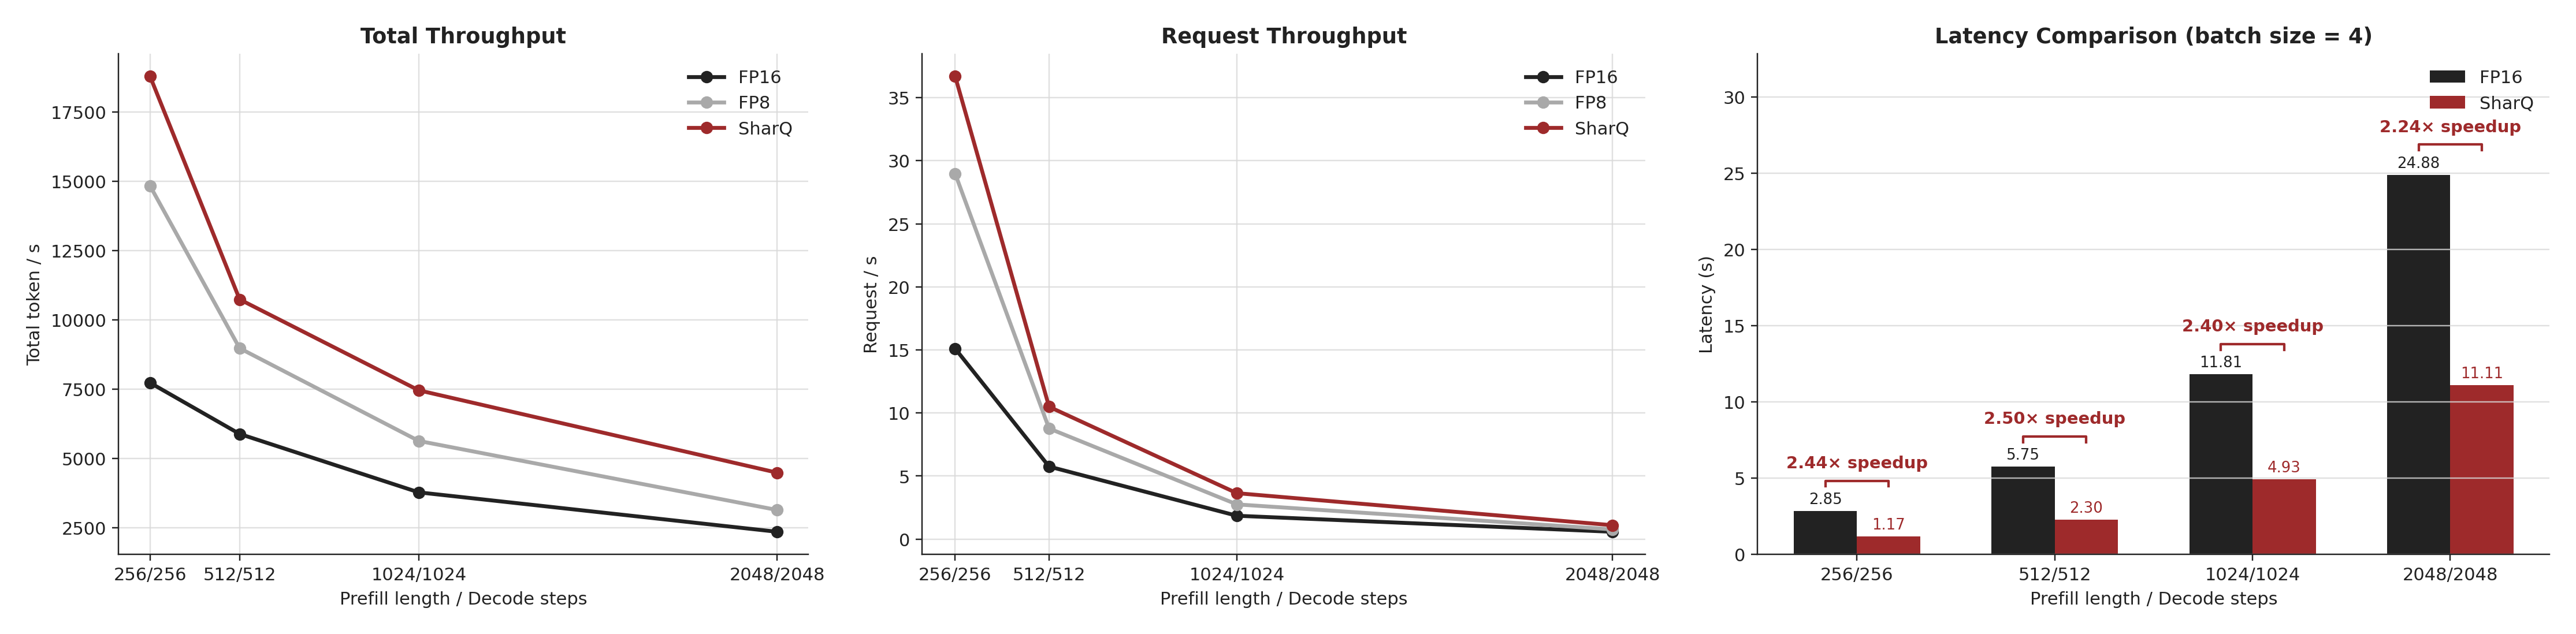
\includegraphics[width=\linewidth]{figures/vllm_efficiency_1x3_red_black.png}
  \caption{vLLM end-to-end efficiency evaluation.}
  \label{fig:vllm-efficiency}
\end{figure}

\subsection{Ablation study}

We conduct two ablation studies to validate the design choices of SharQ.

\textbf{Generalization across FP4 formats.}
Table~\ref{tab:ablation-format} evaluates SharQ on two distinct FP4 numeric
formats: NVFP4 (with 4:8 in-pairs sparsity) and HiF4 (with 2:4 sparsity).
On Qwen3-30B-A3B, SharQ improves both formats consistently. For NVFP4,
WikiText2 perplexity drops from 9.12 to 8.96 and LAMBADA accuracy rises from
62.91\% to 64.41\%. For HiF4, the same pattern holds: perplexity improves from
9.08 to 8.92 and LAMBADA from 63.28\% to 64.08\%. BoolQ accuracy also recovers
toward FP16 in both cases. These results confirm that the decomposition strategy
is format-agnostic and benefits any block-scaled FP4 format paired with
hardware-supported semi-structured sparsity.

\begin{table}[t]
\caption{Effect of SharQ on different FP4 formats (Qwen3-30B-A3B).
Perplexity ($\downarrow$) for WikiText2; accuracy (\%) for others.}
\label{tab:ablation-format}
\centering
\small
\begin{tabular}{@{}l|cccc@{}}
\toprule
Method & Wiki2$\downarrow$ & LAMB. & BoolQ & ARC-E \\
\midrule
FP16       & 8.70 & 64.86 & 88.62 & 79.21 \\
\midrule
NVFP4      & 9.12 & 62.91 & 87.77 & \textbf{79.04} \\
SharQ-NVFP4 & \textbf{8.96} & \textbf{64.41} & \textbf{88.41} & 78.58 \\
\midrule
HiF4       & 9.08 & 63.28 & 87.61 & 76.85 \\
SharQ-HiF4 & \textbf{8.92} & \textbf{64.08} & \textbf{88.07} & \textbf{78.07} \\
\bottomrule
\end{tabular}
\end{table}

\begin{table}[t]
\caption{Ablation on sparse--dense path combinations under NVFP4
(Llama-3.1-8B). ``Sparse'' uses only the sparse path without residual
compensation. ``Dense+Dense'' and ``Sparse+Sparse'' use two paths of the
same type. SharQ combines a sparse backbone with a dense residual.}
\label{tab:ablation-combination}
\centering
\small
\begin{tabular}{@{}l|cccc@{}}
\toprule
Combination & Wiki2$\downarrow$ & MMLU & BoolQ & ARC-E \\
\midrule
Sparse          & 82.95 & 25.78 & 57.03 & 36.74 \\
Dense + Dense   &  \textbf{6.63} & 63.61 & \textbf{81.22} & 76.98 \\
Sparse + Sparse &  6.95 & 61.93 & 79.45 & 77.61 \\
SharQ           &  6.73 & \textbf{63.76} & 80.58 & \textbf{77.74} \\
\bottomrule
\end{tabular}
\end{table}

\textbf{Sparse--dense path combinations.}
Table~\ref{tab:ablation-combination} isolates the contribution of each path
in SharQ by varying the combination of sparse and dense computation under NVFP4
on Llama-3.1-8B. Using only the sparse path without residual compensation
(``Sparse'') is catastrophic: WikiText2 perplexity degrades to 82.95 and MMLU
drops to 25.78\%, confirming that discarding all non-outlier activation
information destroys model quality. ``Dense+Dense'' applies two dense NVFP4 paths
and achieves strong accuracy (WikiText2 6.63, MMLU 63.61), but forgoes the
latency benefit of semi-structured sparse computation. ``Sparse+Sparse'' uses two
sparse paths and yields results comparable to the NVFP4 baseline (WikiText2 6.95,
MMLU 61.93), indicating that doubling the sparse computation without a dense
compensation signal does not recover the sparsification loss. SharQ combines a
sparse backbone with a dense residual, achieving WikiText2 6.73 and MMLU 63.76.
This matches or exceeds the accuracy of the fully dense two-path variant while
retaining the sparse execution path for the backbone, validating that the
asymmetric sparse-plus-dense decomposition is the key to SharQ's
accuracy--efficiency trade-off.

\section{Conclusion}

\section*{References}

{
\small
}

%%%%%%%%%%%%%%%%%%%%%%%%%%%%%%%%%%%%%%%%%%%%%%%%%%%%%%%%%%%%

\appendix
\section{Additional Details}
\section{Supplementary Materials}
\subsection{NVFP4 Data Format}
\label{app:nvfp4}

This section describes the NVFP4 block floating-point format used as the
primary quantization target in our experiments. NVFP4 is a proprietary format
introduced with the NVIDIA Blackwell architecture that improves upon the OCP MXFP4 standard by addressing
two key limitations of prior block-scaled FP4 designs.

\subsubsection{Design rationale}

MXFP4 (OCP Microscaling FP4) uses E2M1 elements with a shared power-of-two
8-bit exponent (E8M0) and a group size of 32, yielding an average storage cost
of 4.25 bits per value. However, the power-of-two constraint on the block scale
cannot guarantee normalization of each group's peak magnitude to the
representable upper bound of E2M1, wasting intra-group dynamic range. NVFP4
introduces two changes to address this:

\begin{enumerate}
\item \textbf{Floating-point block scale.} NVFP4 replaces the power-of-two
E8M0 scale with a fine-grained FP8-E4M3 floating-point scale. This allows the
scale to normalize group peaks more precisely to the upper bound of E2M1,
fully utilizing the intra-group expressive space.

\item \textbf{Smaller group size.} NVFP4 adopts a 16-element group size
(reduced from 32 in MXFP4), raising the average storage cost from 4.25 to 4.5
bits per value but effectively reducing outlier-driven quantization error by
providing finer-grained scaling granularity.
\end{enumerate}

\subsubsection{Format structure}

An NVFP4 block consists of 16 four-bit E2M1 elements sharing a single FP8-E4M3
block scale, for a total storage of $16 \times 4 + 8 = 72$ bits, or 4.5 bits
per value. The E2M1 element format allocates 2 bits to the exponent and 1 bit
to the mantissa (with an implicit leading 1 for normal values), plus 1 sign
bit. The representable nonzero magnitudes in E2M1 are
$\{0.5, 1.0, 1.5, 2.0, 3.0, 4.0, 6.0\}$, with the maximum value being 6 and
special encodings reserved for $\pm 0$ and NaN.

The FP8-E4M3 block scale uses 4 exponent bits (bias 7) and 3 mantissa bits,
providing a scale dynamic range of $[-10, 11]$ in binades (22 binades total).
Combined with the E2M1 element range, the local intra-group dynamic range is
$\log_2(6/0.5) = 3.58$ binades.

\subsubsection{Per-tensor scaling}

Because the E4M3 block scale provides only 22 binades of global dynamic range,
NVFP4 requires an additional software-based per-tensor scaling (PTS) step
before format conversion. PTS normalizes each tensor's peak magnitude to a
target value (typically 2688 for activations) so that the E4M3 scale range is
sufficient to cover the tensor's value distribution. This additional
preprocessing step incurs some overhead during inference but is necessary to
prevent overflow and underflow in the block scale.

\subsubsection{Sparsity support}

On the Blackwell architecture, NVFP4 natively supports 4:8 semi-structured
sparsity in pairs. Within each group of 8 consecutive elements (organized as 4
pairs), the hardware retains 4 elements (2 pairs) and prunes the remaining 4.
This ``in-pairs'' constraint means that sparsity selection operates on pairs of
adjacent elements rather than individual values, which simplifies hardware
metadata encoding while still enabling effective activation sparsity. SharQ
exploits this 4:8 in-pairs pattern as the sparse backbone constraint in its
NVFP4 instantiation.

\subsubsection{Comparison with other FP4 formats}

Table~\ref{tab:nvfp4-comparison} summarizes the key differences between NVFP4
and other block-scaled FP4 formats.

\begin{table}[h]
\caption{Comparison of block-scaled FP4 format designs.}
\label{tab:nvfp4-comparison}
\centering
\small
\begin{tabular}{@{}lccc@{}}
\toprule
Feature & MX4 & MXFP4 & NVFP4 \\
\midrule
4-bit Element       & S1P1       & E2M1  & E2M1 \\
Block Scale Format  & E8M0       & E8M0  & E4M3 \\
Group Size          & 16         & 32    & 16 \\
Storage Cost        & 4.0 bits   & 4.25 bits & 4.5 bits \\
Scale Type          & Power-of-2 & Power-of-2 & Floating-point \\
Significand Precision & 2 bits   & 2 bits & 2 bits \\
Local Dynamic Range & 2.81 binades & 3.58 binades & 3.58 binades \\
Global Dynamic Range & N/A       & N/A   & 22 binades \\
Requires PTS        & No         & No    & Yes \\
\bottomrule
\end{tabular}
\end{table}

NVFP4 achieves better quantization accuracy than MXFP4 by combining the
floating-point scale (which fully utilizes E2M1's representable range) with a
smaller group size (which reduces the impact of outliers within each block).
However, the limited global dynamic range of E4M3 necessitates per-tensor
scaling, and the smaller group size increases metadata overhead. These
trade-offs position NVFP4 as a format optimized for inference accuracy on
current hardware, while formats like HiF4 (Appendix~\ref{app:hif4}) explore
alternative designs with wider dynamic range and lower hardware cost.

\subsection{HiFloat4 (HiF4) Data Format}
\label{app:hif4}

This section provides a detailed description of the HiFloat4 (HiF4) block
floating-point format, which is one of the FP4 numeric formats evaluated in our
ablation study (Table~\ref{tab:ablation-format}). HiF4 was proposed as a
high-fidelity 4-bit BFP format for deep learning inference and training. We
summarize its structure, encoding, and key differences from NVFP4 to make the
paper self-contained.

\subsubsection{Format overview}

A basic HiF4 unit packs 64 four-bit in-group elements together with 32 bits of
shared scaling metadata, resulting in an average storage cost of 4.5 bits per
value (identical to NVFP4). The distinguishing feature of HiF4 is a three-level
scaling hierarchy that captures both inter-group and intra-group dynamic range
variation, improving representational utilization compared with single- or
two-level scaling designs.

%%% PLACEHOLDER: Figure illustrating the HiF4 unit structure %%%
%%% (three-level hierarchy: E6M2 -> E1_8 -> E1_16 -> 64 x S1P2) %%%
% \begin{figure}[t]
%   \centering
%   \includegraphics[width=0.85\linewidth]{figures/hif4_structure.pdf}
%   \caption{Structure of the HiF4 block floating-point format. A single HiF4
%   unit consists of a level-1 E6M2 global base scale, 8 level-2 one-bit
%   micro-exponents (E1\_8), 16 level-3 one-bit micro-exponents (E1\_16), and
%   64 four-bit S1P2 scalar elements.}
%   \label{fig:hif4-structure}
% \end{figure}

\subsubsection{Three-level scaling metadata}

The 32-bit scaling metadata is organized into three hierarchical levels:

\textbf{Level-1: Global base scale (E6M2).}
The first level is a specially designed unsigned 8-bit floating-point format
called E6M2. It assigns 6 bits to the exponent field with a bias of 48 and 2
bits to the mantissa field with one hidden integer bit set to~1. E6M2 encodes
NaN (Not a Number) but does not support infinity or zero; only normal mode is
used. If we denote the unbiased exponent as $E$ and the mantissa as $M$, an
E6M2 value is interpreted as
\begin{equation}
  X = 2^{E} \times 1.M .
  \label{eq:e6m2}
\end{equation}
This scale provides a wide dynamic range across groups (unbiased exponent range
$[-48, 15]$) and normalizes each group's peak magnitude to the representable
upper bound of the remaining hierarchical structure, ensuring full utilization
of the intra-group dynamic range.

\textbf{Level-2: 8-way one-bit micro-exponents (E1\_8).}
The second level consists of 8 one-bit micro-exponents, each shared by 8
consecutive in-group elements. Each E1 bit encodes either 1 or 0, representing
a very fine-grained power-of-two scaling factor ($2^{E1}$ collapses to either
$2$ or $1$). Each level-2 E1 further connects to two adjacent level-3
micro-exponents.

\textbf{Level-3: 16-way one-bit micro-exponents (E1\_16).}
The third level consists of 16 one-bit micro-exponents, each shared by 4
contiguous four-bit elements within its local group. Together with the level-2
micro-exponents, these refine the intra-group dynamic range by capturing local
exponent differences, effectively mitigating the impact of outliers and
suppressing quantization error.

All three levels of scaling metadata occupy 32 bits in total ($8 + 8 + 16$),
distributed over 64 in-group elements, leading to an extra overhead of 0.5 bits
per value.

%%% PLACEHOLDER_ENCODING_TABLES %%%

\subsubsection{Element encoding: S1P2}

HiF4 encodes the 64 four-bit in-group elements using the sign-magnitude S1P2
representation. In the SXPY notation, S denotes the sign bit and P indicates
the binary point; the value X preceding P designates the integer part, and the
value Y following P designates the fractional part. Conceptually, S1P2 is
equivalent to the E1M2 format in floating-point representation. The encoding
details are summarized in Table~\ref{tab:hif4-encoding}.

\begin{table}[h]
\caption{E6M2 and S1P2 encoding details used in HiF4.}
\label{tab:hif4-encoding}
\centering
\small
\begin{tabular}{@{}lcc@{}}
\toprule
Property & Unsigned FP8-E6M2 & Sign-Magnitude S1P2 \\
\midrule
Exponent Bias   & 48              & N/A \\
Unbiased Exp    & $[-48,\;15]$    & N/A \\
Infinity        & N/A             & N/A \\
Zero            & N/A             & $\text{S}0.00_2 = \pm 0.00$ \\
NaN             & $111111\_11_2$  & N/A \\
Max Value       & $111111\_10_2 = 2^{15} \times 1.50$ & $\text{S}1.11_2 = \pm 1.75$ \\
Min Value       & $000000\_00_2 = 2^{-48} \times 1.00$ & $\text{S}0.01_2 = \pm 0.25$ \\
\bottomrule
\end{tabular}
\end{table}

\subsubsection{Value representation}

Based on the three-level hierarchy, each of the 64 real numbers
$\{V_i\}_{i=1}^{64}$ in a HiF4 group can be expressed as follows. If
$\text{E6M2} = \text{NaN}$, then $V_i = \text{NaN}$ for all
$i \in [1, 64]$. Otherwise,
\begin{equation}
  V_i
  =
  \text{E6M2}
  \times
  2^{\left(\{\text{E1\_8}\}_{\lfloor i/8 \rfloor}
    + \{\text{E1\_16}\}_{\lfloor i/4 \rfloor}\right)}
  \times
  \{\text{S1P2}\}_i ,
  \label{eq:hif4-value}
\end{equation}
where $\{\text{E1\_8}\}_j$ ($j \in [1,8]$) and
$\{\text{E1\_16}\}_k$ ($k \in [1,16]$) denote the level-2 and level-3
micro-exponents, respectively. The available intra-group dynamic range of HiF4
is $\log_2(7/0.25) = 4.81$ binades, since the maximum positive value within a
group is $2^{(1+1)} \times 1.75 = 7$ and the minimum positive value is
$2^{(0+0)} \times 0.25 = 0.25$.

\subsubsection{Comparison with NVFP4}

Table~\ref{tab:hif4-vs-nvfp4} compares the key features of HiF4 and NVFP4.
Despite identical average storage costs, HiF4 offers a substantially wider
global dynamic range (69 vs.\ 22 binades), higher significand precision (3 bits
vs.\ 2 bits), and a larger local dynamic range (4.81 vs.\ 3.58 binades). These
properties make HiF4 more robust to outlier-driven quantization error and
reduce the need for software-based per-tensor scaling (PTS) that NVFP4
typically requires.

\begin{table}[h]
\caption{Feature comparison between HiF4 and NVFP4.}
\label{tab:hif4-vs-nvfp4}
\centering
\small
\begin{tabular}{@{}lcc@{}}
\toprule
Feature & HiF4 & NVFP4 \\
\midrule
Storage Overhead       & 4.5 bits/value & 4.5 bits/value \\
Group Size             & 64             & 16 \\
Special Values         & NaN and $\pm 0$ & NaN and $\pm 0$ \\
4-bit Element          & S1P2 (E1M2)   & E2M1 \\
Significand Precision  & 3 bits         & 2 bits \\
Global Base Scale      & E6M2           & E4M3 \\
Max Positive Value     & $2^{18} \times 1.3125$ & $2^{11} \times 1.3125$ \\
Min Positive Value     & $2^{-50}$      & $2^{-10}$ \\
Global Dynamic Range   & $[-50,\;18]$: 69 binades & $[-10,\;11]$: 22 binades \\
Local Dynamic Range    & 4.81 binades   & 3.58 binades \\
\bottomrule
\end{tabular}
\end{table}

\subsubsection{Conversion from BF16 to HiF4}

Algorithm~\ref{alg:bf16-to-hif4} outlines the conversion procedure from a
64-length BF16 vector to a HiF4 unit. The algorithm proceeds in three stages:
(1)~a three-level tree reduction to find local and global peak magnitudes;
(2)~derivation of the three-level hierarchical scaling metadata (E6M2, E1\_8,
E1\_16); and (3)~scaling and quantization of the 64 in-group elements into S1P2
format. All rounding operations use round-half-to-even or
round-half-away-from-zero. The E6M2 reciprocal computation can be efficiently
implemented using only a 4-entry lookup table indexed by the 2-bit mantissa,
combined with simple exponent subtraction.

\begin{algorithm}[h]
\caption{Conversion from BF16 to HiF4}
\label{alg:bf16-to-hif4}
\begin{algorithmic}[1]
\REQUIRE A 64-length BF16 vector $V64$
\ENSURE A HiF4 unit: E6M2, E1\_8, E1\_16, S1P2\_64
\STATE \textbf{// Stage 1: Three-level tree reduction}
\FOR{$i = 1$ to $16$}
  \STATE $V16[i] = \max(|V64[4 \times i - 3 : 4 \times i]|)$
\ENDFOR
\FOR{$i = 1$ to $8$}
  \STATE $V8[i] = \max(V16[2 \times i - 1 : 2 \times i])$
\ENDFOR
\STATE $Vmax = \max(V8)$
\STATE \textbf{// Stage 2: Derive scaling metadata}
\STATE $SF_{BF16} = Vmax \times (1/7)_{BF16}$
  \hfill\COMMENT{High-precision scale factor}
\STATE $\text{E6M2} = \text{BF16\_to\_E6M2}(SF_{BF16})$
  \hfill\COMMENT{Level-1 scale}
\STATE $\text{E6M2\_REC} = \text{E6M2\_REC\_to\_BF16}(\text{E6M2})$
  \hfill\COMMENT{Reciprocal}
\STATE $\text{E1\_8}[i] = (V8[i] \times \text{E6M2\_REC} \geq 4)\ ?\ 1 : 0$
  \hfill\COMMENT{Level-2 scales}
\FOR{$i = 1$ to $16$}
  \STATE $\text{E1\_16}[i] = (V16[i] \times \text{E6M2\_REC} \times 2^{-\text{E1\_8}[\lceil i/2 \rceil]} \geq 2)\ ?\ 1 : 0$
\ENDFOR
\STATE \textbf{// Stage 3: Quantize 64 elements}
\FOR{$i = 1$ to $64$}
  \STATE $V64\_\text{scaled}[i] = V64[i] \times \text{E6M2\_REC} \times 2^{-\text{E1\_8}[\lceil i/8 \rceil]} \times 2^{-\text{E1\_16}[\lceil i/4 \rceil]}$
\ENDFOR
\STATE $\text{S1P2\_64} = \text{BF16\_to\_S1P2}(V64\_\text{scaled})$
  \hfill\COMMENT{Quantize to S1P2}
\end{algorithmic}
\end{algorithm}

For the HiF4 dot product, level-2 and level-3 micro-exponents can be
implemented as simple left-shift operations in hardware. When integrated into
existing 64-length dot-product units originally optimized for 16-bit and 8-bit
formats, HiF4 occupies only approximately one-third the incremental area of
NVFP4 and reduces power consumption by about 10\%, enabling a more area- and
power-efficient implementation for matrix multiplication.

%%% PLACEHOLDER: Figure comparing HiF4 and NVFP4 dot-product compute flow %%%
% \begin{figure}[t]
%   \centering
%   \includegraphics[width=\linewidth]{figures/hif4_dot_product.pdf}
%   \caption{Compute flow of 64-length dot product for HiF4 and NVFP4.
%   HiF4 employs pure integer arithmetic during the reduction from 64 products
%   to a single output, requiring only one small floating-point multiplier and
%   one large integer multiplier at the final accumulation stage.}
%   \label{fig:hif4-dot-product}
% \end{figure}

%%%%%%%%%%%%%%%%%%%%%%%%%%%%%%%%%%%%%%%%%%%%%%%%%%%%%%%%%%%%

\newpage
\input{checklist.tex}

\end{document}
